This section presents the evolution of optical fibre (OF) deployments, from the Points-Of-Presence (POPs) to the end users. POPs are covered in Section~\ref{sec:POPs}.

\subsection{Pilot's deployments}
\label{dep_pilots}

During the second reporting period\footnote{NOTE: Commons for Europe project has three reporting periods: Nov 2012 - Oct 2013, Nov 2012 - Oct 2013 and Nov 2013 - Oct 2014. In this document they can also be referred as fist year (Y1), second year (Y2) and third year (Y3), or simply 2012, 2013 and 2014.}, \emph{Gurb}'s pilot, the most developed of the three pilots, has kept growing steadily in terms of new users connected, in \emph{Vic}'s the PoP has been raised and the initial connections have been made, and in \emph{Rub\'{i}}, a pilot categorised as "blocked" by the end of the first year, new opportunities for the third year have appeared.


\FloatBarrier

\subsubsection{Gurb}
\label{dep_gurb}

In the first OF initiative in guifi.net, where the PoP infrastructure had been risen, put into service and the first deployment iteration made even before Commons for Europe project was started, the second iteration, the deployment expected for the second year, is being carried out as planned -three fourths of the users are already connected and the rest are expected to be connected before the end of the year. The two first deployment iterations have proved that the BuB OF model works for rural areas (i.e. farms and isolated houses). This kind of deployments are essentially aerial. On the contrary, the area of third iteration, the third year's iteration, is a urban area (mostly detached houses with seldom apartment buildings). This deployment the wiring will be done mostly using already existing ducts owned by the local government. The terms for their usage have already been established and the agreements signed.

Table~\ref{tab:gurb} summarises the evolution of the \emph{Gurb}'s pilot during the second year. 

\begin{table}[H]\small
  \begin{center}
    \begin{tabular}{|l|c|}
      \hline
      \multicolumn{2}{|c|}{\textbf{OF deployment of \emph{Gurb}'s Pilot in 2013}} \\
      \hline
      \hline
      New users already connected & 40 \\
      \hline
      Additional users expected by the end of 2013 & 20 \\
      \hline
      Unsubscribed users (vs. 2012) & 0 \\
      \hline
      Km of OF deployed & 20 \\
      \hline
    \end{tabular}
    \caption[Gurb pilot: pilot evolution 2013]{Gurb's OF deployment evolution in 2013.}
    \label{tab:gurb}
  \end{center}
\end{table}

Figure~\ref{fig:gurb_2013_detail} shows the deployment evolution on a map. Red are lines existing before 2013. Blue and cyan are end user and backbone lines made operational in 2013. Green are lines to be executed by the end of 2013. Brown are backbone lines planned for 2014.

\begin{figure}[H]
  \centering
<<<<<<< HEAD:D_5_4_2_report_on_pilots_on_fiber_deployment_b/deployments/deployments.tex
    \begin{tabular}{cc}
      \resizebox{70mm}{!}{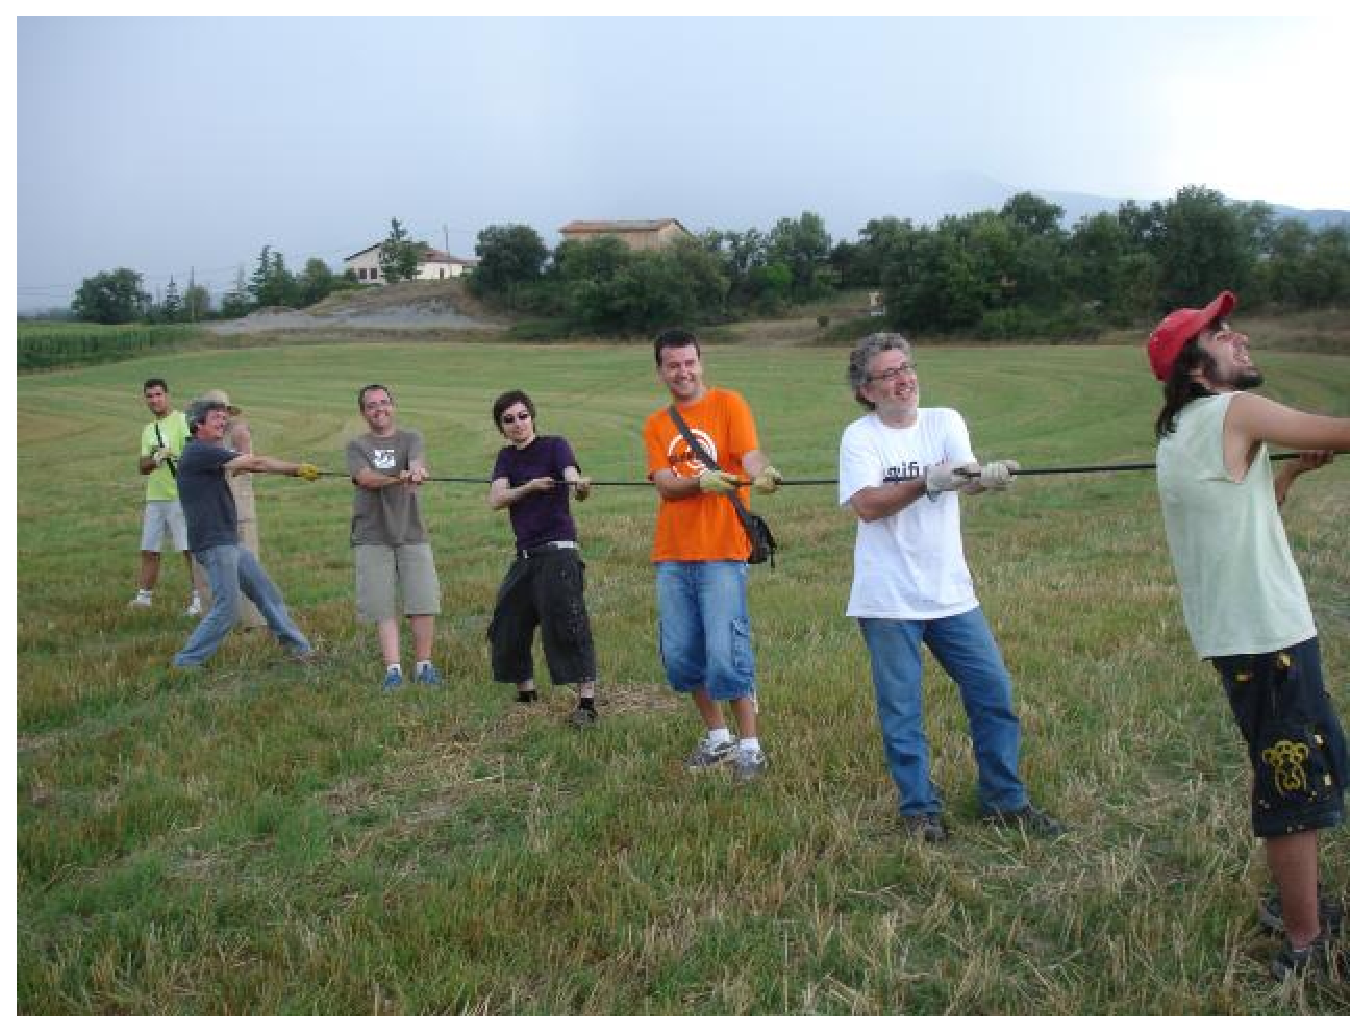
\includegraphics{deployments/figures/Gurb_it1_pic1.eps}} &
      \resizebox{70mm}{!}{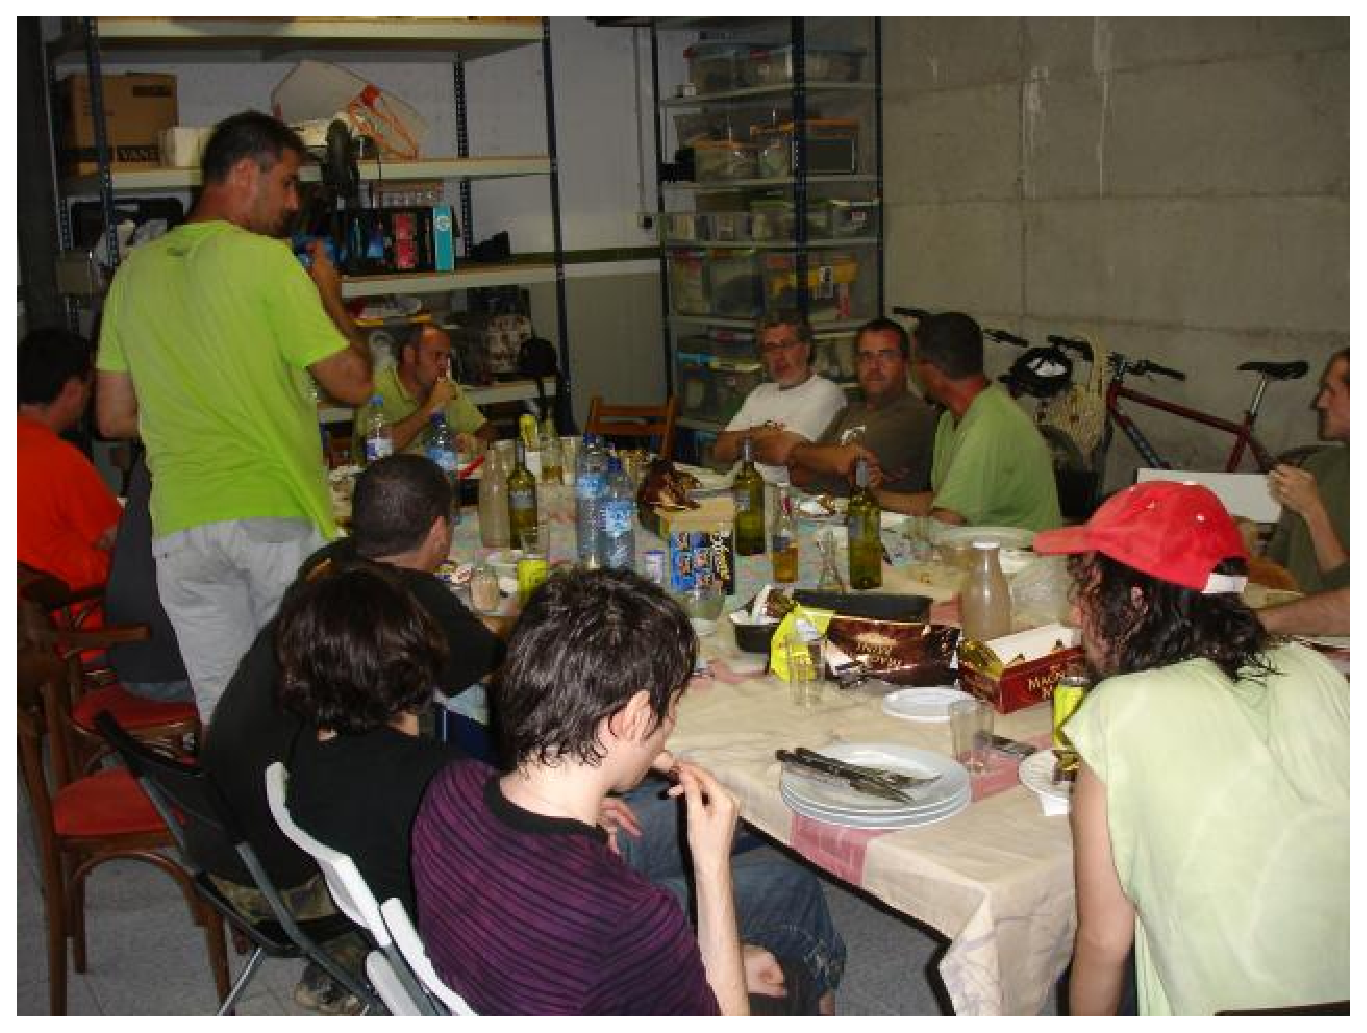
\includegraphics{deployments/figures/Gurb_it1_pic2.eps}} \\
      \resizebox{70mm}{!}{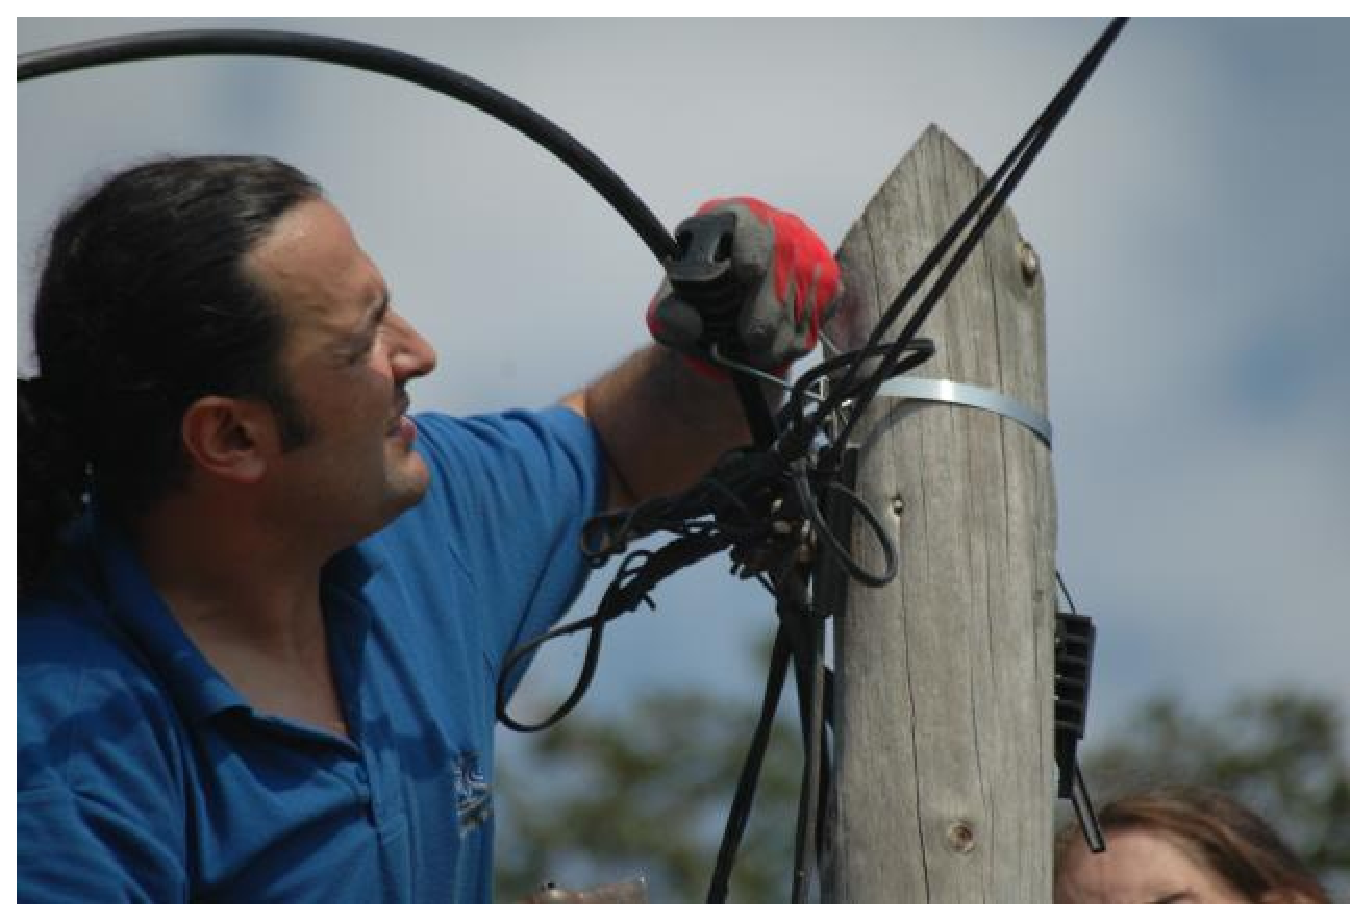
\includegraphics{deployments/figures/Gurb_it1_pic3.eps}} &
      \resizebox{70mm}{!}{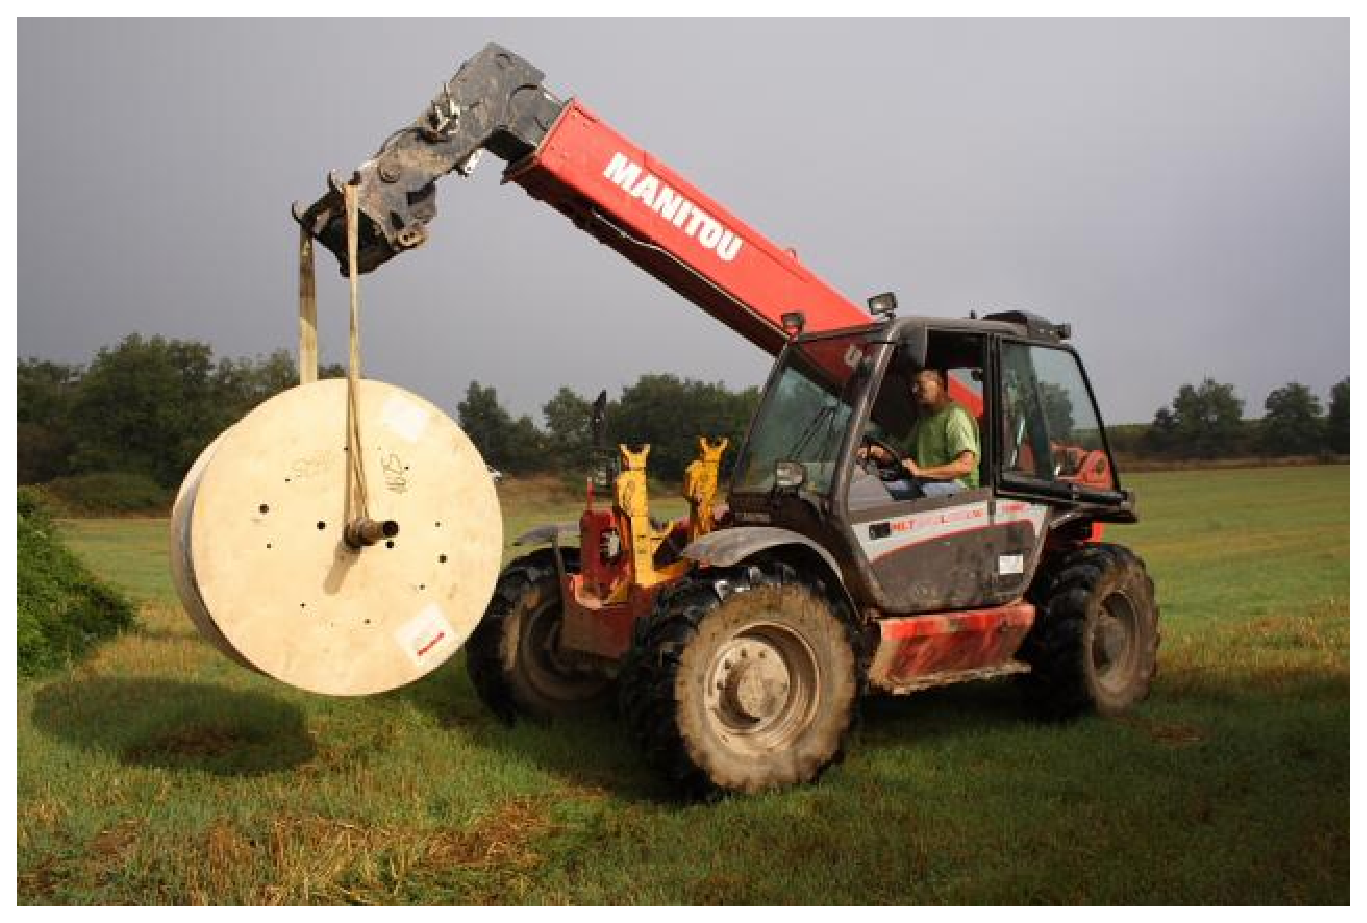
\includegraphics{deployments/figures/Gurb_it1_pic4.eps}} \\
    \end{tabular}
  \caption{OF deployment in Gurb's first iteration. Pictures of the deployment execution, August 2009.}
  \label{fig:gurb_it1_pics}
=======
  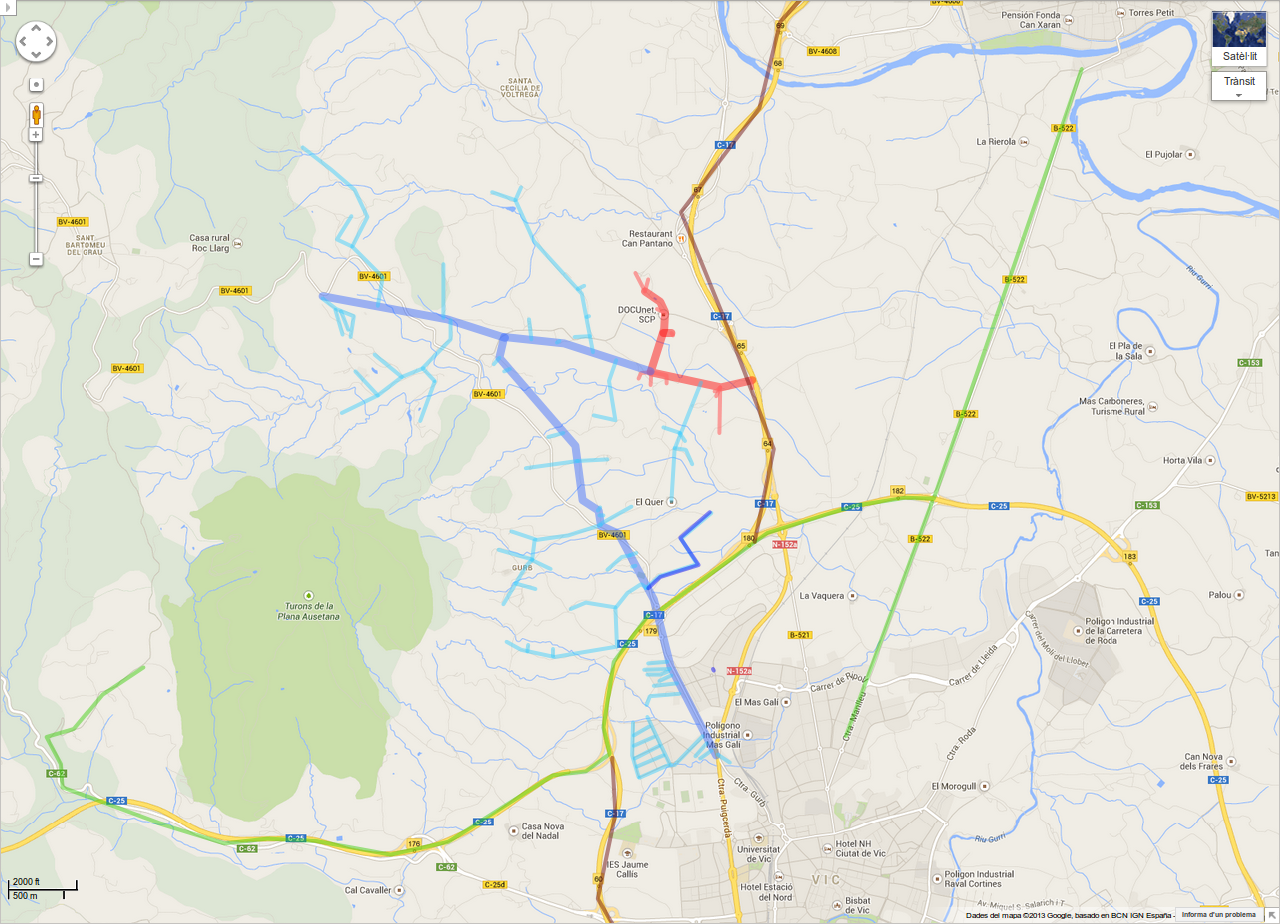
\includegraphics[width=0.95\linewidth]{sect2/figures/gurb_2013_detail.png}
  \caption[Gurb pilot: OF deployment map of 2nd and 3rd iterations]{OF deployment in Gurb's second and third iterations.}
  \label{fig:gurb_2013_detail}
>>>>>>> rbaig/master:D_5_4_2_report_on_pilots_on_fiber_deployment_b/sect2/deployments.tex
\end{figure}

Figure~\ref{fig:gurb_user_con} depicts how end user connections are made.

\begin{figure}[H]
  \centering
<<<<<<< HEAD:D_5_4_2_report_on_pilots_on_fiber_deployment_b/deployments/deployments.tex
  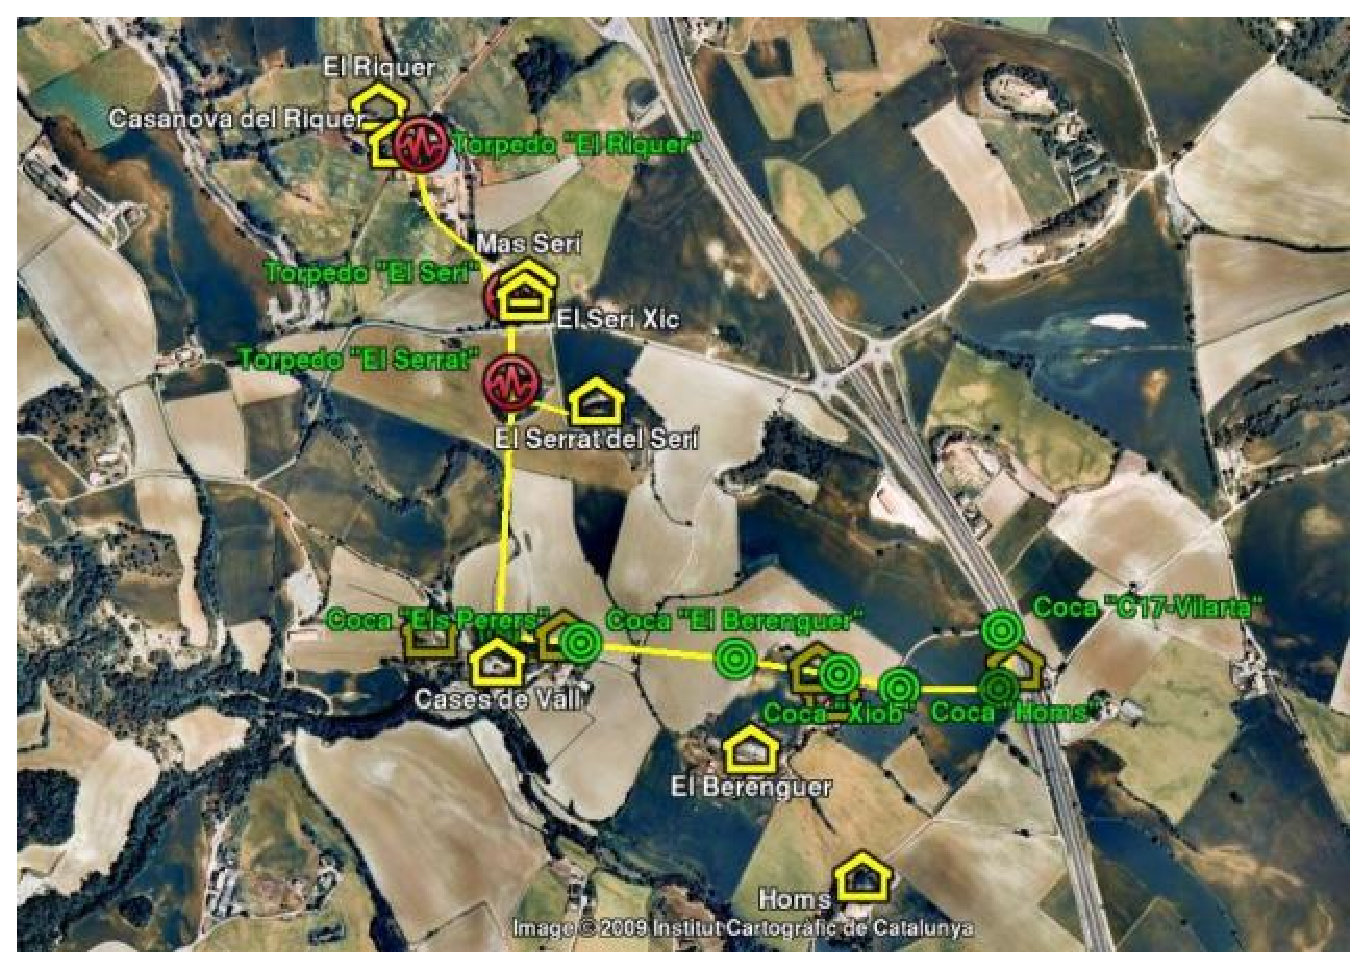
\includegraphics[scale=.65]{deployments/figures/Gurb_it1_map.eps} 
  \caption{OF deployment in Gurb's first iteration. Map. Executed in 2009.}
  \label{fig:gurb_it1_map}
=======
    \begin{tabular}{cc}
      \resizebox{0.465\linewidth}{!}{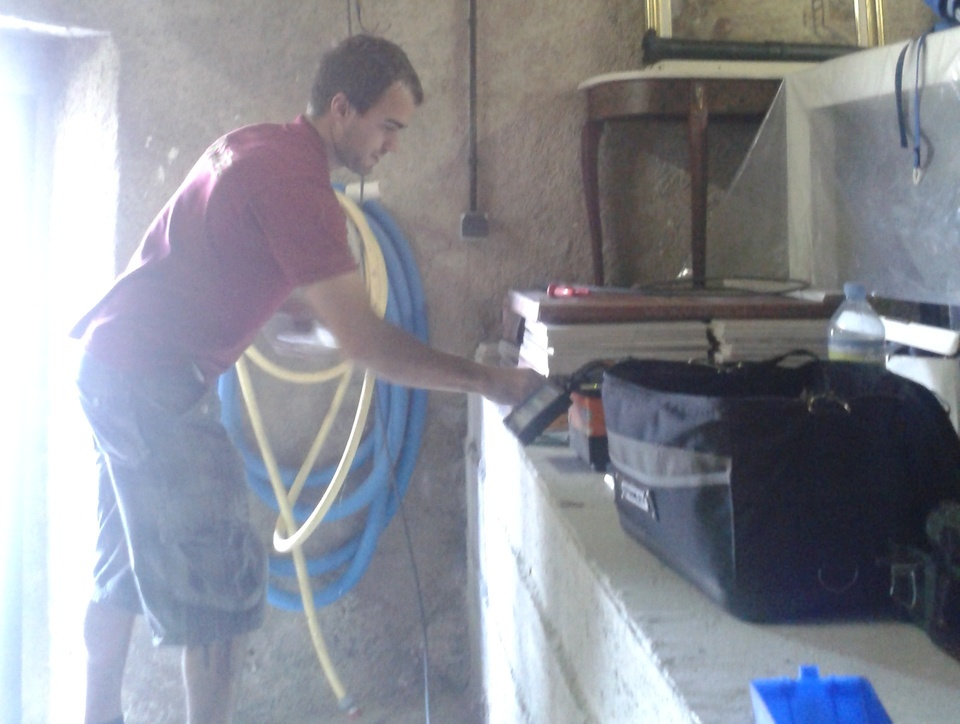
\includegraphics{sect2/figures/user_con1.jpg}} &
      \resizebox{0.465\linewidth}{!}{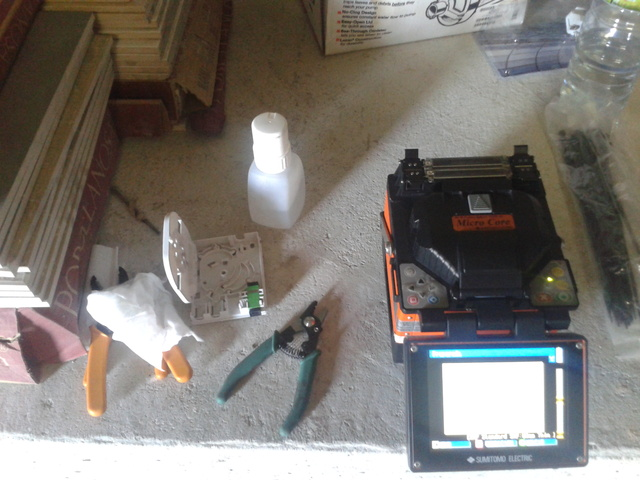
\includegraphics{sect2/figures/user_con2.jpg}} \\
      \resizebox{0.465\linewidth}{!}{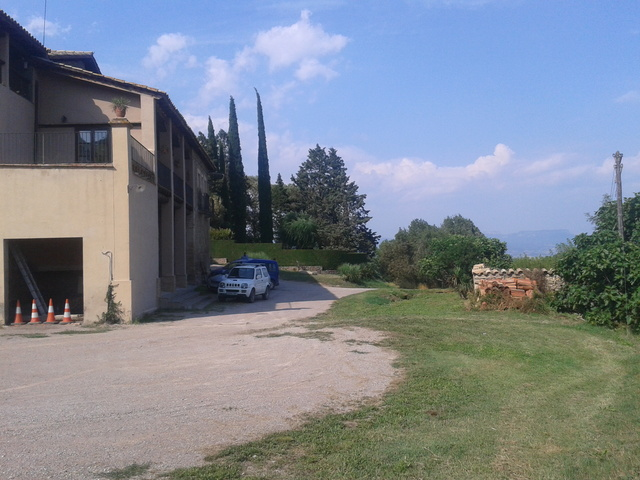
\includegraphics{sect2/figures/user_con3.jpg}} &
      \resizebox{0.465\linewidth}{!}{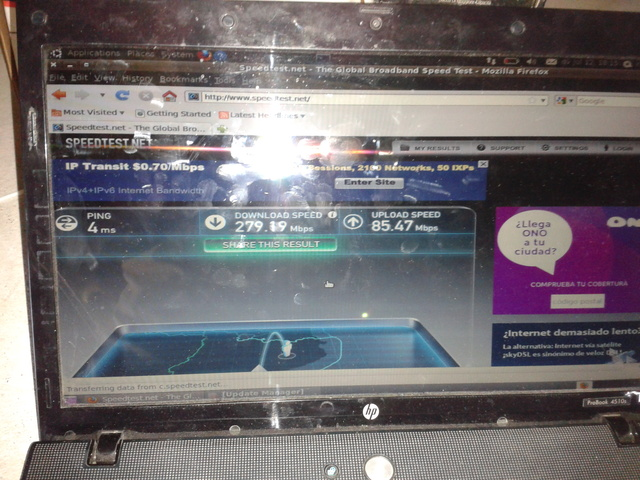
\includegraphics{sect2/figures/user_con4.jpg}} \\
    \end{tabular}
  \caption[Gurb pilot: Connecting a farm]{Connecting a farm. Top left: Preparing the fibre splicer. Top right: The fibre splicer and the additional tools needed. Bottom left: The house being connected. Bottom right: Speed test results.}
  \label{fig:gurb_user_con}
>>>>>>> rbaig/master:D_5_4_2_report_on_pilots_on_fiber_deployment_b/sect2/deployments.tex
\end{figure}

Figure~\ref{fig:gurb_2013_transit} shows the average daily traffic\footnote{All traffic figures are 95-percentile.}. It increases as the number of connected end users increase. The cut of mid September corresponds to a sabotage that took place in September the 11th\footnote{September the 11th is the Catalan national day. It is suspected that the sabotage was directly related to this fact as part of the reaction of the independence process of Catalonia.}.

\begin{figure}[H]
  \centering
<<<<<<< HEAD:D_5_4_2_report_on_pilots_on_fiber_deployment_b/deployments/deployments.tex
  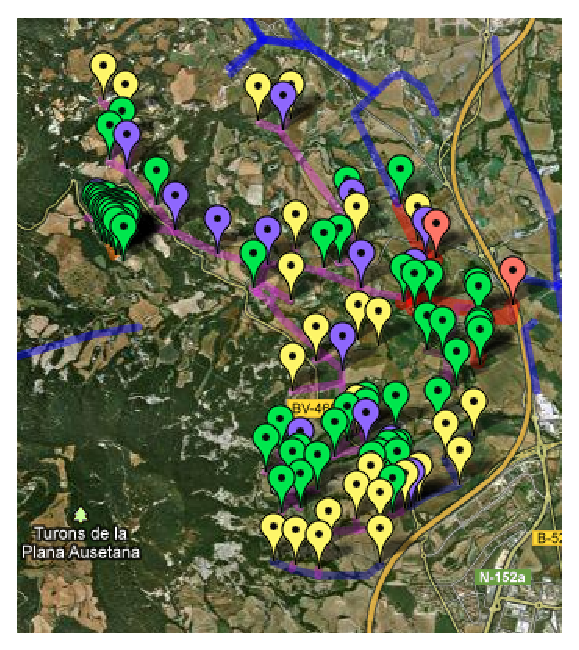
\includegraphics[scale=1.3]{deployments/figures/Gurb_it2_map.eps} 
  \caption{OF deployment in Gurb's fist iteration. Map. Blue spots are the \emph{Passive Optical Splitters}, green spots are homes connected as of the beginning of December 2012, yellow spots are homes to be connected by the end of this iteration.}
  \label{fig:gurb_it2_map}
=======
  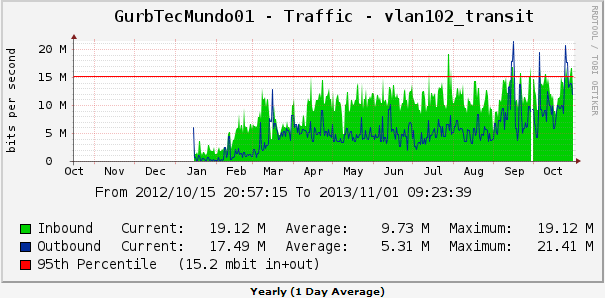
\includegraphics[width=0.95\linewidth]{sect2/figures/gurb_2013_transit.png}
  \caption[Gurb pilot: Network traffic 2013]{Gurb's pilot network traffic 2013.}
  \label{fig:gurb_2013_transit}
>>>>>>> rbaig/master:D_5_4_2_report_on_pilots_on_fiber_deployment_b/sect2/deployments.tex
\end{figure}


\FloatBarrier
\subsubsection{Vic}
\label{dep_vic}

This urban deployment is the result of the collaboration of individuals, industries and social services. In the first iteration a primary and a secondary school, a hospital and chemical industry together with a dozen of dwelling houses have been connected. It is expected that the number of connections will significantly increase in 2014.

Figure~\ref{fig:vic_2013_detail} is the map of the second (2013) and the third (2014) iterations. Green are end user and backbone lines already operational. Orange are lines to be executed by the end of 2013. Red are lines planned for 2014.

\begin{figure}[H]
  \centering
<<<<<<< HEAD:D_5_4_2_report_on_pilots_on_fiber_deployment_b/deployments/deployments.tex
    \begin{tabular}{cc}
      \resizebox{70mm}{!}{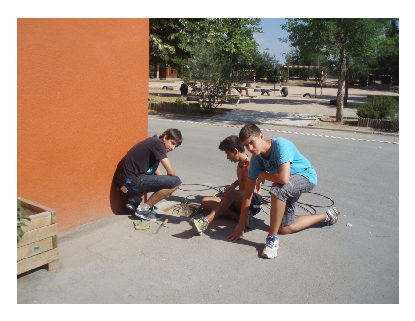
\includegraphics{deployments/figures/Vic_it1_pic1.eps}} &
      \resizebox{70mm}{!}{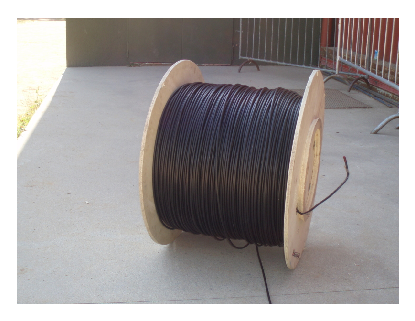
\includegraphics{deployments/figures/Vic_it1_pic2.eps}} \\
      \resizebox{70mm}{!}{
\includegraphics{deployments/figures/Vic_it1_pic3.eps}} &
      \resizebox{70mm}{!}{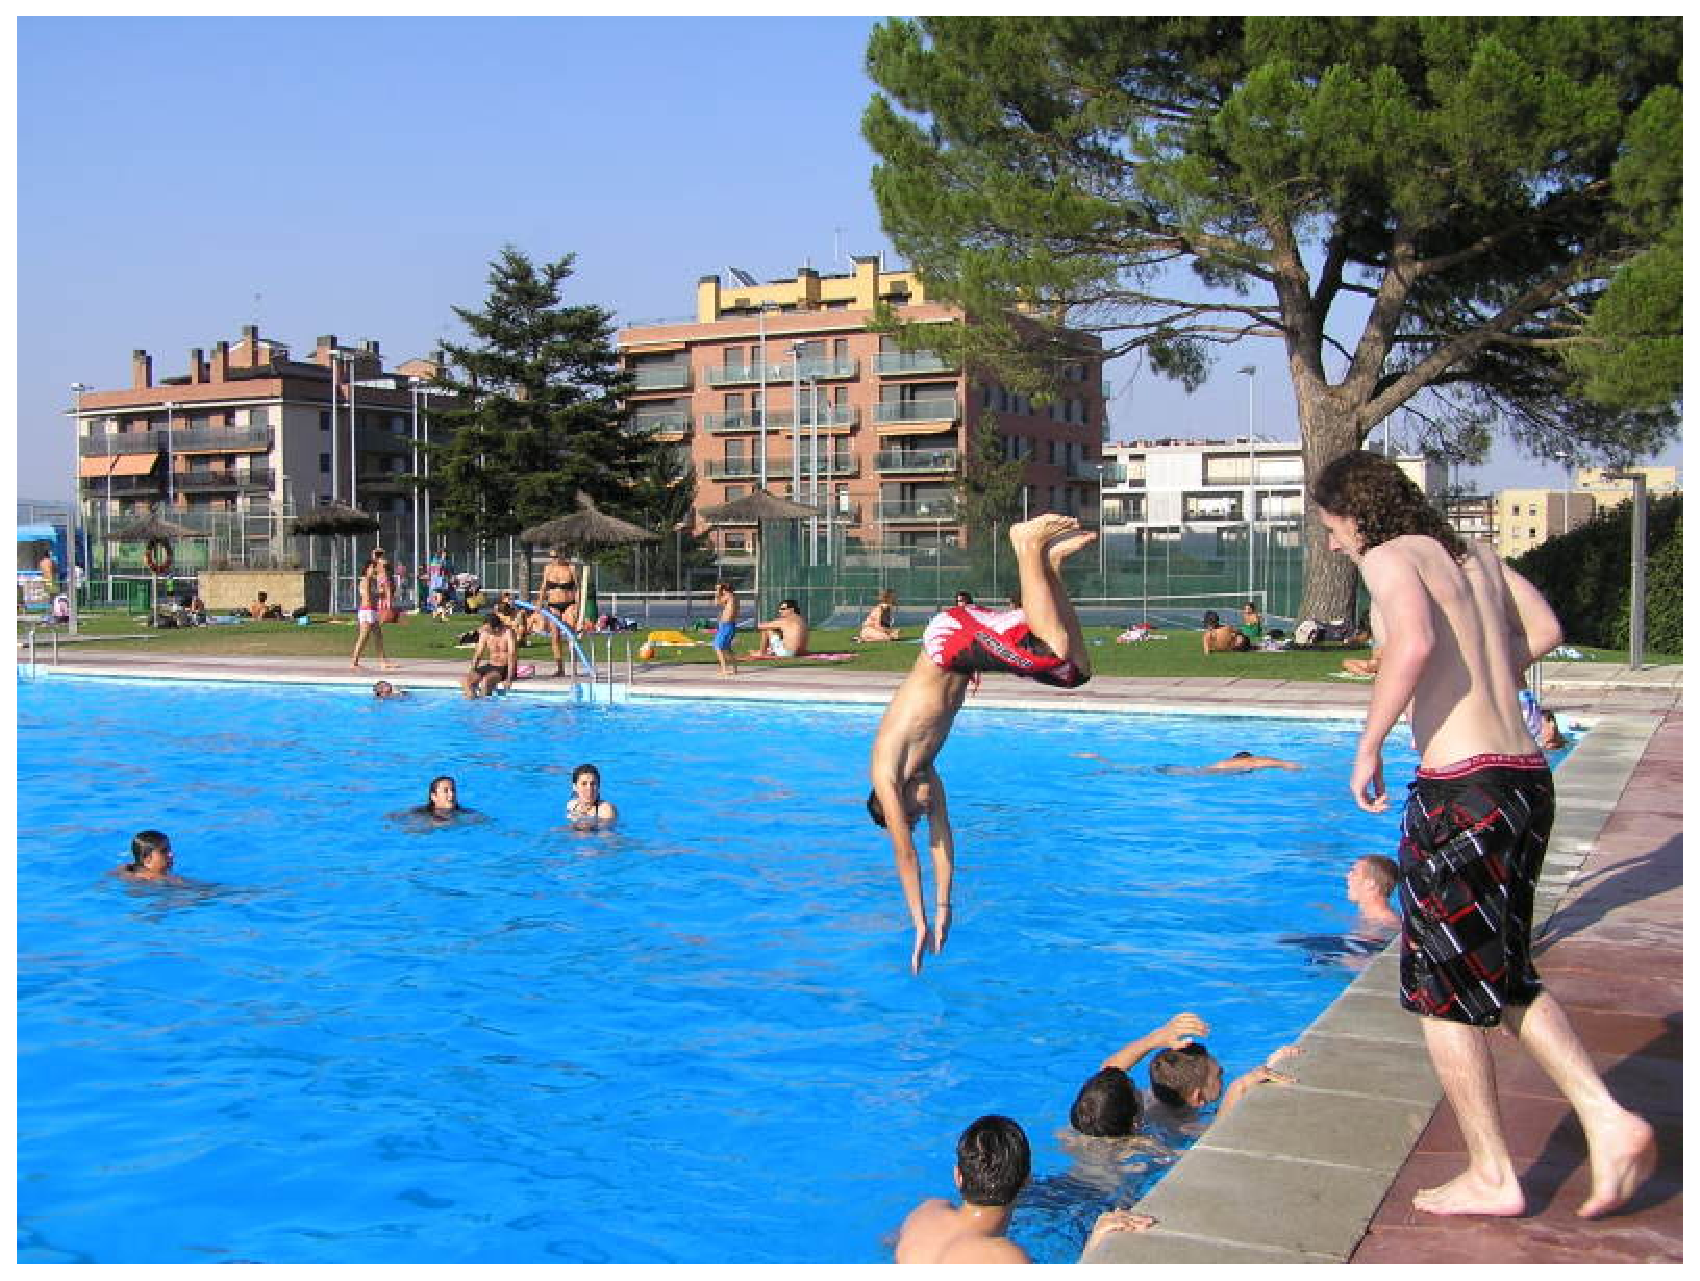
\includegraphics{deployments/figures/Vic_it1_pic4.eps}} \\
    \end{tabular}
  \caption{OF deployment in Vic's first iteration. Pictures of the deployment execution during the summer camp, August 2012.}
  \label{fig:vic_it1_pics}
=======
  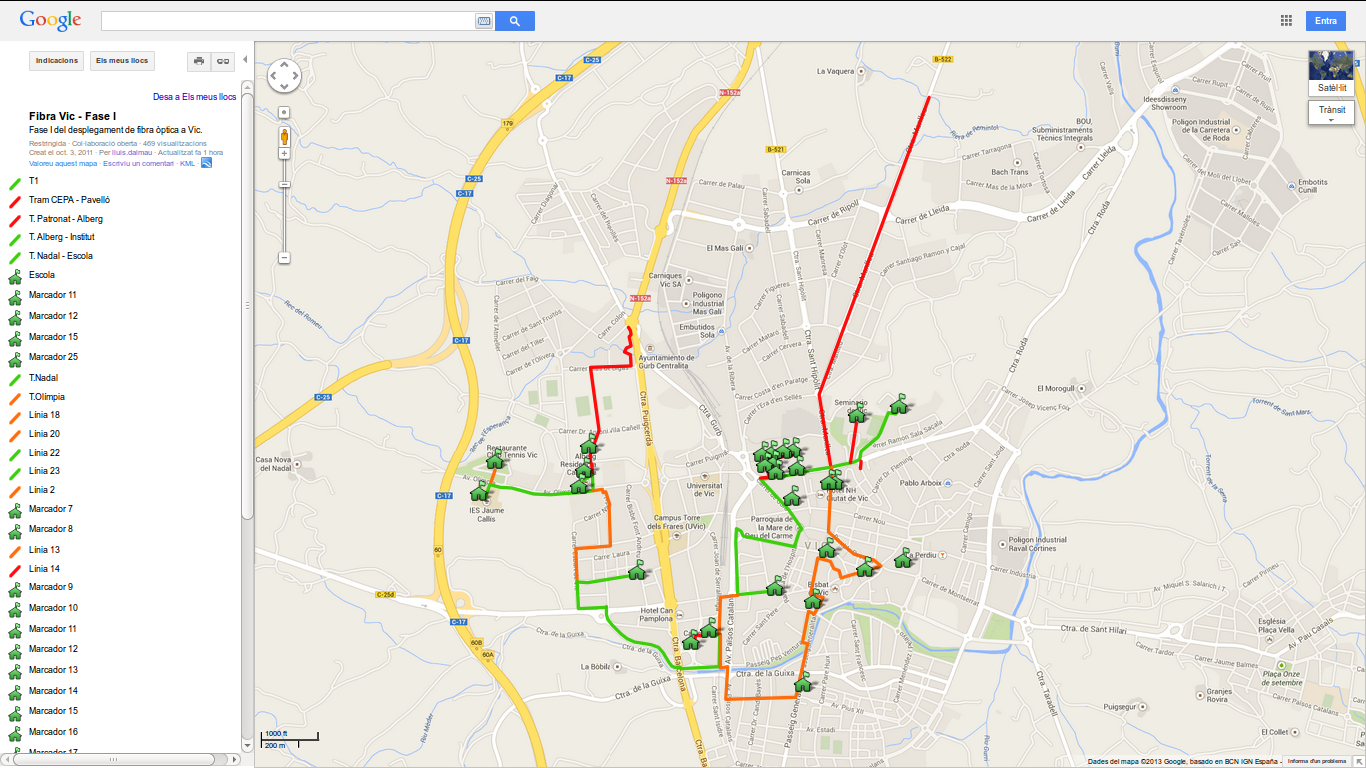
\includegraphics[width=0.95\linewidth]{sect2/figures/vic_2013_detail.png}
  \caption[Vic pilot: OF deployment map of 2nd and 3rd iterations]{OF deployment in Vic's second and third iterations.}
  \label{fig:vic_2013_detail}
>>>>>>> rbaig/master:D_5_4_2_report_on_pilots_on_fiber_deployment_b/sect2/deployments.tex
\end{figure}


\begin{figure}[H]
  \centering
<<<<<<< HEAD:D_5_4_2_report_on_pilots_on_fiber_deployment_b/deployments/deployments.tex
  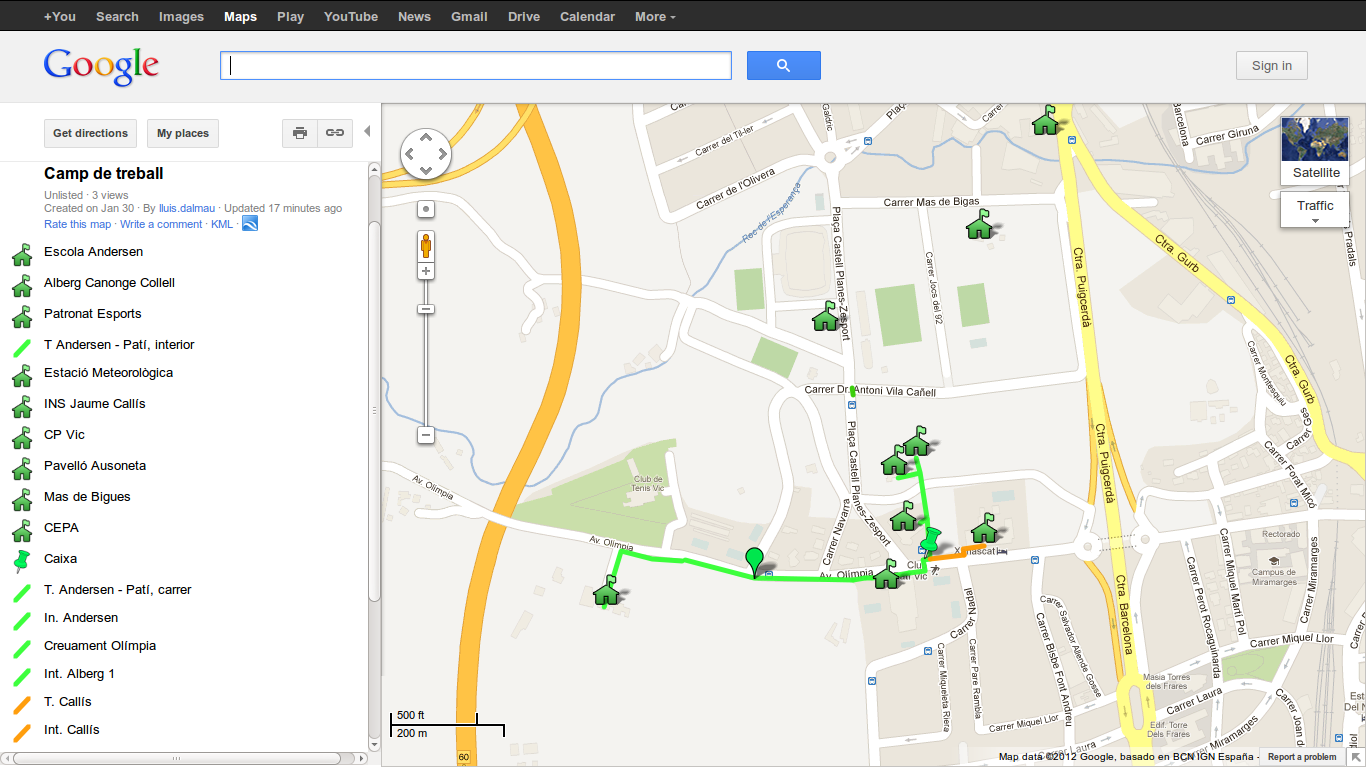
\includegraphics[scale=.33]{deployments/figures/Vic_summer_camp_2012.eps} 
  \caption{OF deployment in Vic's first iteration. Executed in 2012. Result of a teenager's summer camp.}
  \label{fig:vic_sc12}
=======
    \begin{tabular}{cc}
      \resizebox{0.465\linewidth}{!}{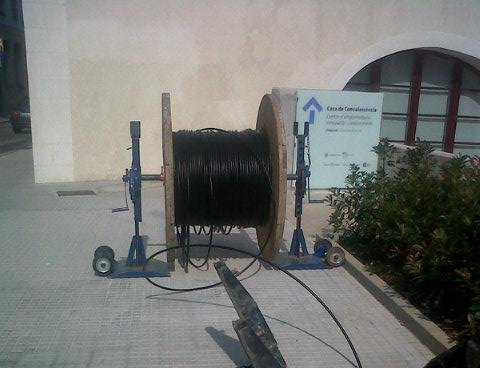
\includegraphics{sect2/figures/20130702_vic_fibra_optica_guifi_net.jpeg}} &
      \resizebox{0.465\linewidth}{!}{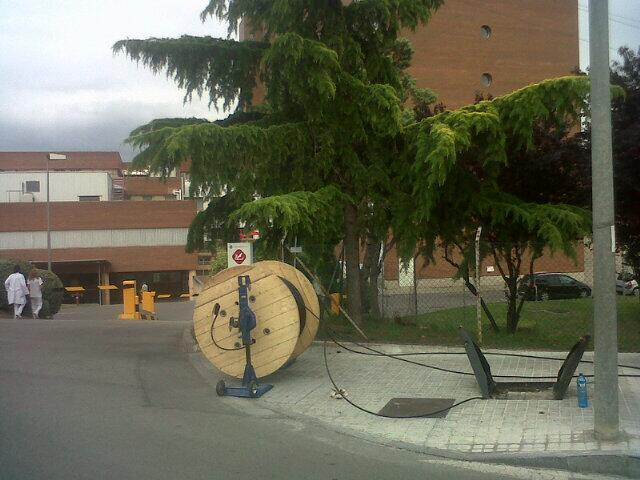
\includegraphics{sect2/figures/20130703_vic_fibra_optica_guifi_net.jpeg}} \\
      \resizebox{0.465\linewidth}{!}{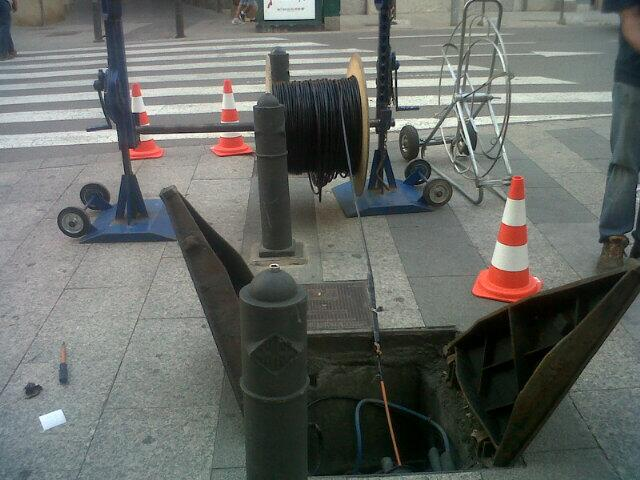
\includegraphics{sect2/figures/20130718_vic_fibra_optica_guifi_net.jpeg}} &
      \resizebox{0.465\linewidth}{!}{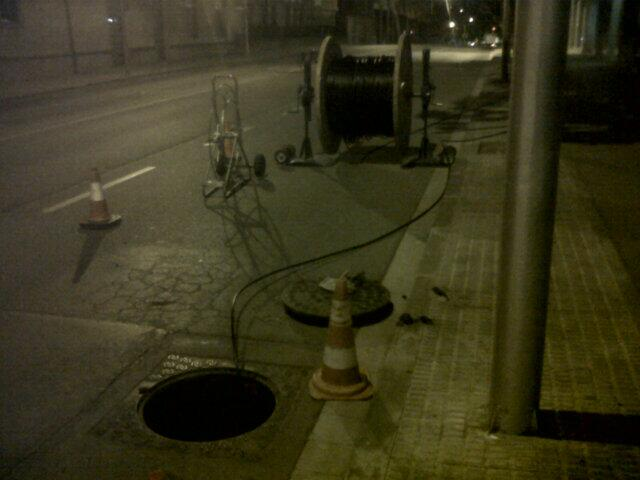
\includegraphics{sect2/figures/20130704_vic_fibra_optica_guifi_net.jpeg}} \\
    \end{tabular}
  \caption[Vic pilot: Connecting a hospital in an urban area]{Connecting a hospital in an urban area. Top left: The fibre reel close to the Hospital's main entrance. Top right: Already outside the Hospital venue. Bottom left: Along the streets. Bottom right: Working until late at night.}
  \label{fig:vic_user_con}
>>>>>>> rbaig/master:D_5_4_2_report_on_pilots_on_fiber_deployment_b/sect2/deployments.tex
\end{figure}


\begin{figure}[H]
  \centering
<<<<<<< HEAD:D_5_4_2_report_on_pilots_on_fiber_deployment_b/deployments/deployments.tex
  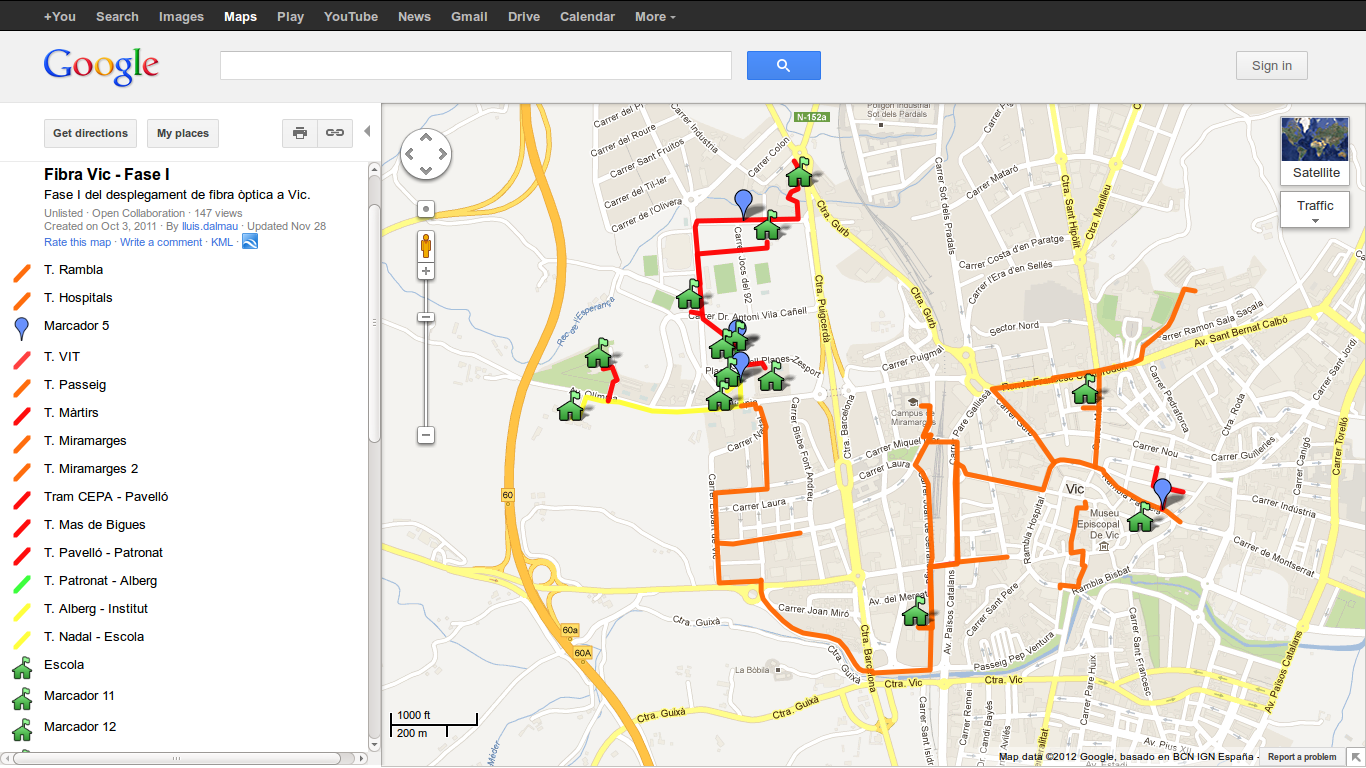
\includegraphics[scale=.33]{deployments/figures/Vic_iteration1.eps} 
  \caption{OF deployment in Vic second iteration. Planned for 2013.}
  \label{fig:vic_it1}
=======
  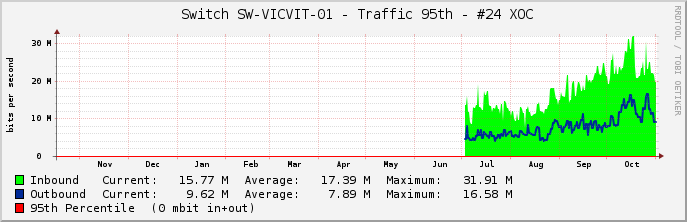
\includegraphics[width=0.95\linewidth]{sect2/figures/vic_2013_transit.png}
  \caption[Vic pilot: Network traffic 2013]{Vic's pilot network traffic 2013.}
  \label{fig:vic_2013_transit}
>>>>>>> rbaig/master:D_5_4_2_report_on_pilots_on_fiber_deployment_b/sect2/deployments.tex
\end{figure}


\FloatBarrier
\subsubsection{Rub\'{i}}
\label{dep_rubi}

As already detailed in the first report, by the end of the first year this pilot was considered to be in a blocked state. In 2013 on the one hand the traditional ISPs have continued deploying their own OF, but on the other hand new opportunities to deploy BuB OF appeared. Indeed, in June a person from the city advised by the local government contacted the guifi.net Foundation to get further information about the BuB model and to discuss on the viability of setting up a consumers cooperative ISP. At the moment it is a work in progress to be consolidated during the year 2014. Nonetheless it looks promising because this person has a wide experience in such kind of cooperatives (she had played a relevant role in the creation of the renewable energies consumer cooperative Som Energia\footnote{\url{http://www.somenergia.coop/welcome-to-som-energia}}) and because the initiative is viewed as favourably by the local government and has its support.


\FloatBarrier
\subsection{Other deployments}
\label{dep_other}

Aside from the selected pilots there are other on-going FO initiatives in side guifi.net at various stages of maturity. The consolidated (those that already have a PoP up and operational) ones are:

\begin{itemize}
\item Masquefa
\item Igualda
\item Manresa
\item Aldea
\item Tortosa
\end{itemize}

<<<<<<< HEAD:D_5_4_2_report_on_pilots_on_fiber_deployment_b/deployments/deployments.tex
% Table~\ref{tab:other_deployments} summarises them.
%
%\begin{table}[htbp]
%  \centering
%    \begin{tabular}{|p{2cm}|p{6cm}|p{6cm}|}
%      \hline \textbf{Project} & \textbf{Status} & \textbf{Comments} \\ \hline \hline
%      Taradell & First iteration executed in 2012 & Interconnection of a secondary school with guifi.net local POP \\
%      Igualda & First iteration planned for 2013 & Connection of many homes expected \\ \hline
%    \end{tabular}
%  \caption{Other deployments.}
%  \label{tab:other_deployments}
%\end{table}
=======
It is expected that other initiatives will consolidate in 2014.
>>>>>>> rbaig/master:D_5_4_2_report_on_pilots_on_fiber_deployment_b/sect2/deployments.tex
